\documentclass[12pt, a4paper]{report}
\usepackage{graphicx, array, amsthm, amssymb, amsmath, algorithm, algpseudocode, float, xcolor, thmtools, thmbox, matlab-prettifier, exercise}
\usepackage[english]{babel}

\makeatletter
\renewcommand\thmbox@headstyle[2]{\bfseries #1}
\makeatother
\newtheorem[style=M,bodystyle=\normalfont]{theorem}{Theorem}
\newtheorem[style=M,bodystyle=\normalfont]{corollary}{Corollary}
\newtheorem[style=M,bodystyle=\normalfont]{lemma}{Lemma}
\newtheorem[style=M,bodystyle=\normalfont]{definition}{Definition}


\title{Image Analysis And Computer Vision\\ \textit{Theory}}
\author{Christian Rossi}
\date{Academic Year 2023-2024}

\begin{document}

\maketitle

\newpage

\begin{abstract}
    The topics of the course are: 
    \begin{itemize}
        \item Introduction.
        \item Camera sensors: transduction, optics, geometry, distortion
        \item Basics on Projective geometry: modelling basic primitives (points, lines, planes, conic sections, quadric surfaces) and projective spatial transformations and  projections.
        \item Camera geometry, and single view analysis: calibration, image rectification, localization of 3D models.
        \item Multi-view analysis: 3D shape reconstruction, self-calibration, 3D scene understanding.
        \item Linear filters and convolutions, space-invariant filters, Fourier Transform, sampling and aliasing. 
        \item Nonlinear filters: image morphology and morphology operators (dilate, erode, open, close), median filters.
        \item Edge detection and feature detection techniques. Feature matching and feature tracking along image sequences.
        \item Inferring parametric models from noisy data (including outliers), contour segmentation, clustering, Hough Transform, Ransac (random sample consensus). 
        \item Applications: object tracking, object recognition, classification.
    \end{itemize}
\end{abstract}

\newpage

\tableofcontents

\newpage

\chapter{Optical Sensors}
    \section{Photocamera}
    \begin{definition}
    The \emph{photocamera} is an optical sensor; this means that produces data using electric transducers. It uses an optical system that select the direction of the incoming light at each 
    element of its screen made with millions of photosensitive elements. Most of the actual cameras can capture up to 30-60 frames per second. 
    \end{definition}
    For simplicity, we suppose that the optical system of a photocamera is a single lens that is:
    \begin{itemize}
        \item Spherical: the lens is obtained by intersecting two spheres. 
        \item Thin: the distance between the center of the two spheres is almost identical to the sum of the diameter of them. 
        \item Small angles: the light forms small inclination angles with the optical axis.
    \end{itemize}
    This simplifies the computation of the path of the ray crossing the lens. In fact, the refraction of the light when crossing a border between two media is given by the Snell's law: 
    \[\dfrac{\sin{\theta_2}}{\sin{\theta_1}}=\dfrac{n_1}{n_2}\]
    where: 
    \begin{itemize}
        \item $\theta_1$ and $\theta_2$ are the angles between the normal at the surface and the direction of the light ray, respectively before and after crossing the border. 
        \item $n_1$ and $n_2$ are the refraction indexes of the two materials.
    \end{itemize}
    \begin{figure}[H]
        \centering
        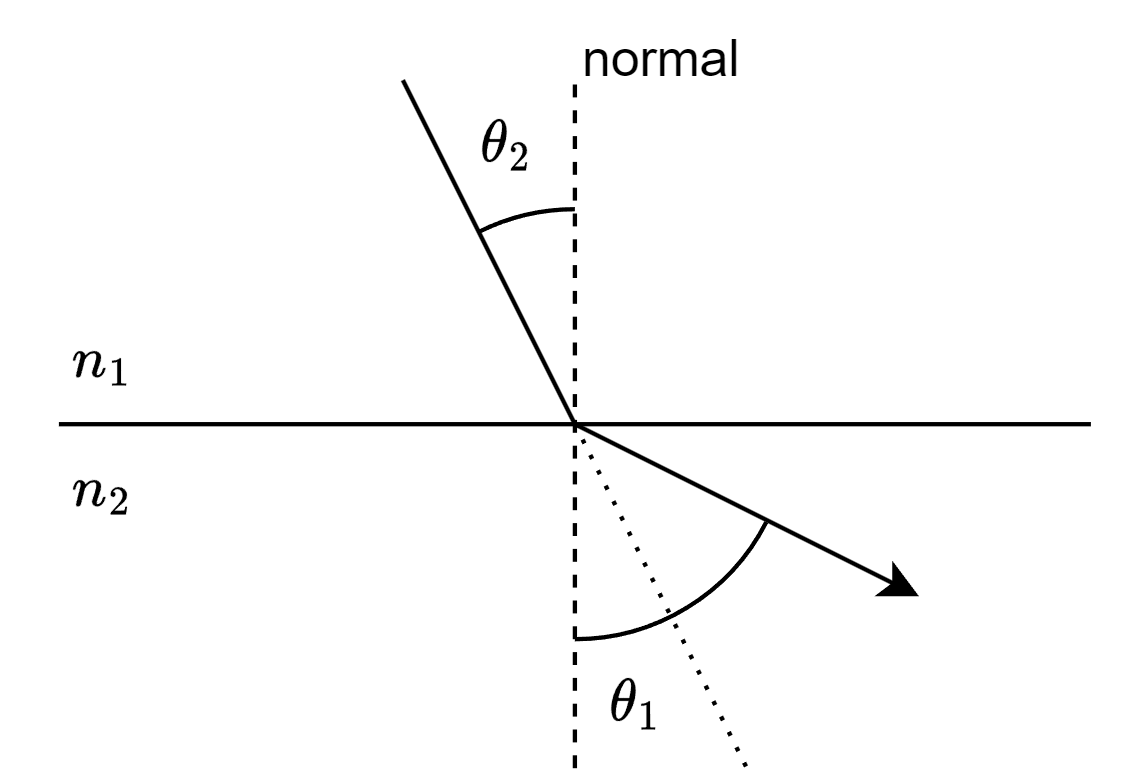
\includegraphics[width=0.5\linewidth]{images/refraction.png}
        \caption{Snell's law}
    \end{figure}
    \begin{definition}
        The \emph{optical axis} is the straight line that connects the center of the two spheres that are used to form the lens. 
    \end{definition}
    The angles of a ray passing through the centers of the spheres can be calculated as follows: 
    \[\alpha_1=\dfrac{y_1}{\rho_1} \:\:\:\:\:\: \alpha_2=-\dfrac{y_2}{\rho_2}\]
    \begin{figure}[H]
        \centering
        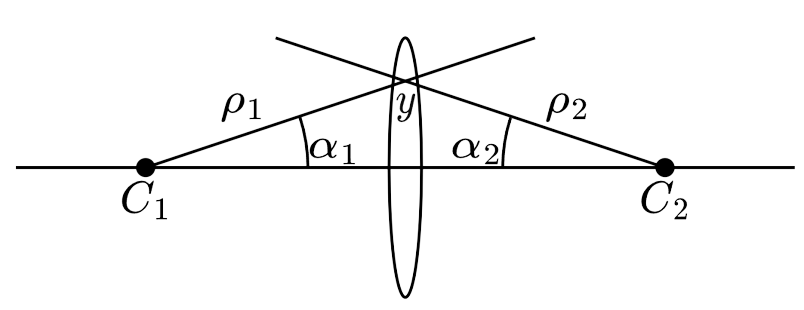
\includegraphics[width=0.5\linewidth]{images/y.png}
    \end{figure}
    Since we have a simplified lens, it is possible to say that:
    \[y_1=y_2=y\]
    
    \section{Light rays deviation}
    \begin{figure}[H]
        \centering
       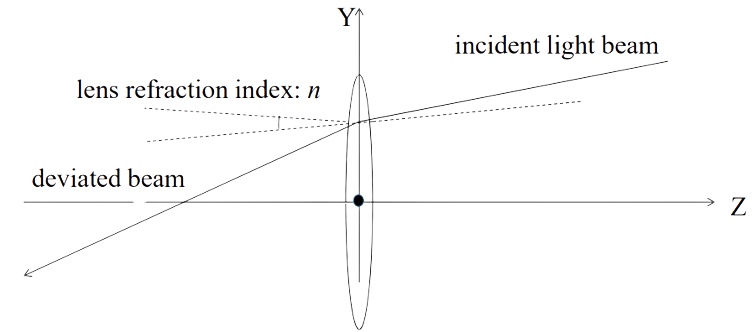
\includegraphics[width=0.5\linewidth]{images/ray.png}
   \end{figure}
    Given a lens with refraction $n$ we have that the following equations are valid:
    \[\dfrac{\theta-\alpha_1}{\theta^{'}-\alpha_1} \Rightarrow \dfrac{\sin{(\theta-\alpha_1)}}{\sin{(\theta^{'}-\alpha_1)}}=n\]
    \[\dfrac{\theta^{''}-\alpha_2}{\theta^{'}-\alpha_2} \Rightarrow \dfrac{\sin{(\theta^{''}-\alpha_2)}}{\sin{(\theta^{'}-\alpha_2)}}=n\]
    where:
    \begin{itemize}
        \item $\theta$ is the angle before the lens. 
        \item $\theta^{'}$ is the angle in the lens (not visible in the image). 
        \item $\theta^{''}$ is the angle after the lens.
    \end{itemize}
    Comparing the two equations it is possible to find the difference between the input angle $\theta$ and the output angle $\theta^{''}$ that is: 
    \[\delta \theta=y(n-1)\left( \dfrac{1}{\rho_1} + \dfrac{1}{\rho_2}\right)\]
    It is possible to see that the first term $(n-1)$ is due to the matter of the lens and the second $\left( \frac{1}{\rho_1} + \frac{1}{\rho_2}\right)$ depend on the curvature 
    of the surface. 

    \section{Focalization of parallel light rays}
    \begin{figure}[H]
        \centering
        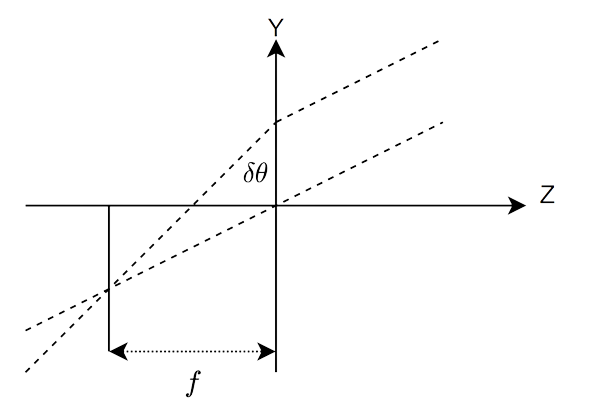
\includegraphics[width=0.5\linewidth]{images/focalization.png}
    \end{figure}
    In the image we have one ray that passes through the center of the lens and the other that passes in another point, but it is parallel to the first one. So we have that: 
    \begin{itemize}
        \item $Y=0$: the deviation of the ray is null and proceed without being deviated. 
        \item $Y=f \cdot \delta \theta \Rightarrow f=\dfrac{1}{(n-1)\left( \dfrac{1}{\rho_1} + \dfrac{1}{\rho_2}\right)}$. 
    \end{itemize}
    This means that all the rays that proceed in parallel meets in one common point on the focal point $Z$, with a distance from the $Y$ axis equal to: 
    \[Z=-f\]

    \section{Path of a light ray}
    To find the projection of a light ray crossing a lens in any position we need to:
    \begin{enumerate}
        \item Draw a line parallel to the selected ray and that passes through the center of the lens. 
        \item Intersect the line with the focal plane.
        \item The ray will go from the point in which it crosses the lens to the point found on the focal plane. 
    \end{enumerate}
    \begin{figure}[H]
        \centering
        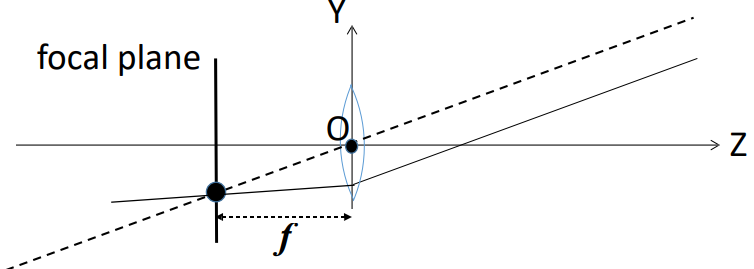
\includegraphics[width=0.5\linewidth]{images/path.png}
        \caption{Path of a light ray through a lens}
    \end{figure}

    \section{Pin-hole camera}
    To have a focussed image we need that every ray hits the focal plane of the camera in exactly one pixel. To obtain this we need that the distance between the lens and
    the source of the ray $Z(P)$ must be much greater than the lens aperture $a$ (at least $1000\times$). In this way we can place the screen at distance $Z$ from the lens. If all they rays
    respect this constraint they will be all parallel for the lens and the image will be on focus. The camera that we have defined so far is called pin-hole camera and needs:
    \begin{enumerate}
        \item Thin spherical lens. 
        \item Small angles.
        \item $Z(P) \gg a$.
        \item $Z=f$.
    \end{enumerate}

    \section{From real world to 2D images}
    The images are in a 2D plane while the real world is in three dimensions. So, a picture have less information than the original subject in the real world. In fact, the space 
    projection of space in a 2D image is a perspective projection, that is: 
    \begin{itemize}
        \item Nonlinear.
        \item Not shape-preserving.
        \item Not length-ratio preserving. 
    \end{itemize}
    Due to the triangle equality we have that:
    \[x=f \dfrac{X}{Z} \:\:\:\:\:\: y=f \dfrac{Y}{Z}\]
    The only way to avoid this information loss is to take a picture of a planar scene on plane parallel to image plane, so we need to have 
    \[Z=Z_0=\textnormal{constant}\]
    \begin{figure}[H]
        \centering
        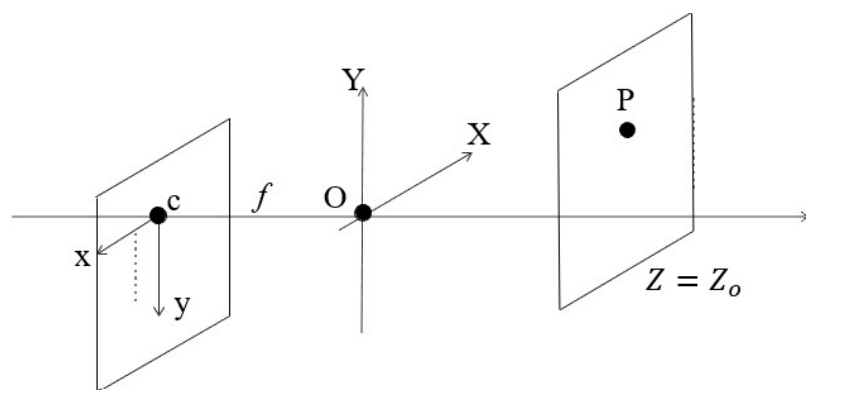
\includegraphics[width=0.5\linewidth]{images/Z0.png}
    \end{figure}
    In this case the only difference between reality and projection will be the down scaling, while the other dimensions are preserved: 
    \[x=f \dfrac{X}{Z_0}=kX \:\:\:\:\:\: y=f \dfrac{Y}{Z_0}=kY \]
    
    \section{Perspective and vanishing point}
    If we decide to choose all the lines parallel to the direction parameters $\begin{bmatrix} \alpha & \beta & 1 \end{bmatrix}$ we obtain the following system: 
    \[
        \begin{cases}
            X = X_0 + \alpha Z  \\
            Y = Y_0 + \beta Z   \\
            Z = 1 \cdot Z
        \end{cases}
    \]
    All these lines can be projected in the 2D image with the triangle equality in the following way: 
    \[x=f \dfrac{X}{Z} = f \dfrac{X_0 + \alpha Z}{Z} = f\alpha + \dfrac{X_0}{Z}\]
    \[y=f \dfrac{Y}{Z} = f \dfrac{Y_0 + \beta Z}{Z}  = f\beta  + \dfrac{Y_0}{Z}\]
    We now want to find the image of the point at the infinity of these lines, so we obtain the point: 
    \[\begin{bmatrix} f\alpha & f\beta \end{bmatrix}\]
    that is independent of $X_0$ and $Y_0$. So, we have that all parallel lines have the same image if their points at the infinity.
    \begin{definition}
        The image of the point at the infinity of the lines is called \emph{vanishing point}. 
    \end{definition}
    So, we have that all the lines that are parallel in the real world will project onto concurrent lines in the image. 
    \begin{figure}[H]
        \centering
        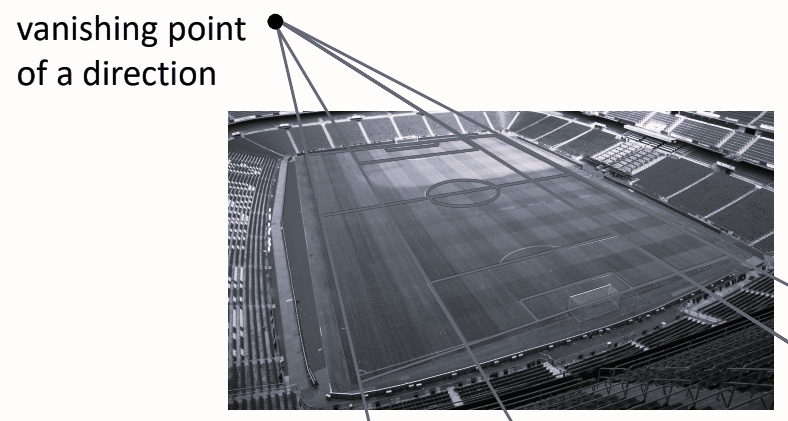
\includegraphics[width=0.6\linewidth]{images/vanishingpoint.png}
        \caption{Example of vanishing point}
    \end{figure}

\newpage

\chapter{Planar Projective Geometry}
    \section{Introduction}
    The elements needed to define a planar geometry are: point, lines, conics and dual conics. The possible transformations in this type of geometry are: projectivities, 
    affinities, similarities and isometries. 

    \section{Points}
    The points can be defined in Cartesian coordinates by defining a euclidean plane with his origin. In this way every point is defined unambiguously with two Cartesian 
    coordinates $(x,y)$. 

    To analyze images it is better to use homogeneous coordinates. To define this type of coordinates we need to construct a 3D space with $x,y,w$ axis. So, now to define a point
    we have to assign three values. This means that every number can be represented in infinite ways by changing the value of $w$. The correlation between Cartesian
    and homogeneous coordinates is the following: 
    \[
    \textbf{x} =
    \begin{bmatrix}
        x \\
        y \\
        w 
    \end{bmatrix}
    =w
    \begin{bmatrix}
        X \\
        Y \\
        1 
    \end{bmatrix}
    \]
    So we have that a vector $\textbf{x} = \begin{bmatrix} x \\ y \\ w \end{bmatrix}$ and all its nonzero multiples $\lambda \begin{bmatrix} x \\ y \\ w \end{bmatrix}$, including
    $\begin{bmatrix} x/w \\ y/w \\ 1 \end{bmatrix}$, represent the point of Cartesian coordinates $\begin{bmatrix} X \\ Y \end{bmatrix}=\begin{bmatrix} x/w \\ y/w\end{bmatrix}$
    on the euclidean plane. This type of representation has the homogeneity property:  any vector $\textbf{x}$ is equivalent to all its nonzero multiples $\lambda \textbf{x}, 
    \lambda \neq 0$, since they represent the same point. The null vector does not represent any point.
    \begin{definition}
        The \emph{projective plane} is defined as:
        \[\mathbb{P}^2=\{{\begin{bmatrix} x & y & w \end{bmatrix}}^T \in \mathbb{R}^3\}-\{{\begin{bmatrix} 0 & 0 & 0 \end{bmatrix}}^T\}\]
    \end{definition}
    \begin{example}
        The origin of the plane is defined as:
        \[{\begin{bmatrix} 0 & 0 & 1 \end{bmatrix}}^T\]
        A generic point in heterogeneous coordinates can be transformed into a couple of Cartesian coordinate with a simple division. The point:
        \[{\begin{bmatrix} 0 & 8 & 4 \end{bmatrix}}^T\]
        in Cartesian coordinate is equal to: 
        \[{\begin{bmatrix} x/w & y/w  \end{bmatrix}}^T=\begin{bmatrix} 0/4 & 8/4 \end{bmatrix}=\begin{bmatrix} 0 & 4 \end{bmatrix}\]
    \end{example}
    Consider the point $\textbf{x}=\begin{bmatrix} x \\ y \\ w \end{bmatrix}$ and let $w$ slowly drop to $0$ starting from $w=1$. As $w$ decreases, the point will move along a 
    constant direction $\begin{bmatrix} x & y \end{bmatrix}$, with increasing distance from the origin. As $w$ tends to $0$, this points tends to the infinity along the direction 
    $\begin{bmatrix} x & y \end{bmatrix}$. 
    \begin{definition}
        The point \[\textbf{x} = \begin{bmatrix} x \\ y \\ w \end{bmatrix}\] is called the \emph{point at the infinity along the direction} $\begin{bmatrix} x & y \end{bmatrix}$. 
    \end{definition}
    Points at the infinity, who represent directions, are not part of the euclidean plane: they are extra points, well-defined within the projective plane. So, in general we have
    that the projective plane is the euclidean plane with also the points at the infinity. 

    \section{Lines}
    In the euclidean plane a line is defined as: 
    \[aX+bY+c=0\]
    In the heterogeneous plane the lines are defined as: 
    \[a\dfrac{x}{w}+b \dfrac{y}{w}+c=0 \Longrightarrow ax+by+cw=0\]
    This equation can be also represented using two vectors called respectively $\textbf{l}^T$ and $\textbf{x}$:
    \[\begin{bmatrix} a & b & c \end{bmatrix} \begin{bmatrix} x \\ y \\ w \end{bmatrix}=0\]
    where the vector $\textbf{l}={\begin{bmatrix} a & b & c \end{bmatrix}}^T$ and all its nonzero multiples represent a line. This type of representation has the homogeneity
    property: any vector $\textbf{l}$ is equivalent to all its nonzero multiples $\lambda \textbf{l}, \lambda \neq 0$, since they represent the same line. $a,b,c$ are called 
    homogeneous parameters of the line. 

    As for numbers, there is an infinite number of equivalent representations for a single line, namely all nonzero multiples of the unit normal vector. The null vector does not
    represent any lines.
    \begin{definition}
        The \emph{projective dual plane} is defined as: 
        \[\mathbb{P}^2=\{{\begin{bmatrix} a & b & c \end{bmatrix}}^T \in \mathbb{R}^3\}-\{{\begin{bmatrix} 0 & 0 & 0 \end{bmatrix}}^T\}\]
    \end{definition}

    There are three important remarks: 
    \begin{enumerate}
        \item If the third parameter is null, ${\textbf{l}=\begin{bmatrix} a & b & 0 \end{bmatrix}}^T$, then the line goes through point $\begin{bmatrix} 0 & 0 \end{bmatrix}$. 
        \item Within the euclidean plane, direction $\begin{bmatrix} a & b \end{bmatrix}$ is normal to the line \\ ${\textbf{l}=\begin{bmatrix} a & b & c \end{bmatrix}}^T$. 
        \item Two lines ${\textbf{l}=\begin{bmatrix} a & b & c \end{bmatrix}}^T$ and ${\textbf{l}=\begin{bmatrix} a & b & c^{'} \end{bmatrix}}^T$ are parallel: their common 
            direction is $[b,-a]$. 
    \end{enumerate}
    \begin{example}
        The Cartesian axes are defined as: 
        \[\textbf{l}_x=\begin{bmatrix} 0 \\ 1 \\ 0 \end{bmatrix} \:\:\:\:\:\: \textbf{l}_y=\begin{bmatrix} 1 \\ 0 \\ 0 \end{bmatrix}\]
    \end{example}
    The incidence relation of a line $\textbf{l}^T\textbf{x}=0$ is defined when the point $\textbf{x}$ is on the line $\textbf{l}$ or the line $\textbf{l}$ goes through the 
    point $\textbf{x}$. 
    \begin{definition}
        The line \[\begin{bmatrix} 0 & 0 & 1 \end{bmatrix} \begin{bmatrix} x \\ y \\ w \end{bmatrix}=\textbf{w}=0\] is called the \emph{line at the infinity} $\textbf{l}_{\infty}={\begin{bmatrix} 0 & 0 & 1 \end{bmatrix}}^T$. 
    \end{definition}
    Since the dot product is commutative, also the incidence relation is commutative. This is called the principle of duality between points and lines. 
    Given the lines $\textbf{l}_1^T$ and $\textbf{l}_2^T$, the intersection can be found by imposing: 
    \[\begin{bmatrix} \textbf{l}_1^T \\ \textbf{l}_2^T \end{bmatrix} \textbf{x} = \begin{bmatrix} 0 \\ 0 \end{bmatrix}\]
    that is equal to find the right null space of the first column vector. 
    \[\textbf{x}=\textbf{RNS}\left( \begin{bmatrix} \textbf{l}_1^T \\ \textbf{l}_2^T \end{bmatrix} \right)\]
    The system found is under determined, so there is only one intersection point between two lines (that can be represented in infinite ways in homogeneous coordinates). Note that 
    the vector $\textbf{x}$ is orthogonal to both lines, so in the 2D projective geometry can be found with the cross product: 
    \[\textbf{x}=\textbf{l}_1 \times \textbf{l}_2\]
    \begin{example}
        Suppose we have two parallel lines $\textbf{l}_1={\begin{bmatrix} a & b & c_1 \end{bmatrix}}^T$ and 
        $\textbf{l}_2={\begin{bmatrix} a & b & c_2 \end{bmatrix}}^T$. The point that is common to both points can be found with the system: 
        \[
            \begin{cases}
                ax+by+c_1w=0 \\
                ax+by+c_2w=0
            \end{cases}
        \]
        So the solution will be ${\textbf{x}=\begin{bmatrix} b & -a & 0 \end{bmatrix}}^T$ that is the point at the infinity along the direction of both lines. 
    \end{example}
    The line through two points can be found with the dual of the previous problem, that is: 
    \[\begin{bmatrix} \textbf{x}_1^T \\ \textbf{x}_2^T \end{bmatrix} \textbf{l} = \begin{bmatrix} 0 \\ 0 \end{bmatrix}\]
    that in 2D become: 
    \[\textbf{l}=\textbf{x}_1 \times \textbf {x}_2\] 
    \begin{example}[Property]
        The point $\textbf{x}$ given by the linear combination $\textbf{x}=\alpha\textbf{x}_1+\beta\textbf{x}_2$ of two points $\textbf{x}_1$ and $\textbf{x}_2$ is on the 
        line $\textbf{l}$ through $\textbf{x}_1$ and $\textbf{x}_2$. 
    \end{example}
    \begin{proof}
        The line $\textbf{l}$ through both points satisfies $\textbf{l}^T\textbf{x}_1=0$ and  $\textbf{l}^T\textbf{x}_2=0$. By adding $\alpha$ times the first 
        equation to $\beta$ times the second one, we obtain: 
        \[0=\textbf{l}^T\left( \alpha\textbf{x}_1+\beta\textbf{x}_2 \right)=\textbf{l}^T\textbf{x}=0\]
    \end{proof}
    This proves that there is also a duality between colinear and concurrent. 
    \begin{theorem}[duality principle]
        For any true sentence containing the words: point, line, is on and goes through there is a dual sentence (also true) obtained by substituting, in the previous one, each 
        occurrence of: 
        \begin{itemize}
            \item Point $\Leftrightarrow$ line. 
            \item Is on $\Leftrightarrow$ goes through.
            \item Colinear $\Leftrightarrow$ concurrent. 
        \end{itemize}
    \end{theorem}
    Within the euclidean plane, $\begin{bmatrix} a & b \end{bmatrix}$ is the direction normal to the line $\textbf{l}={\begin{bmatrix} a & b & c \end{bmatrix}}^T$. Since we have that
    the angle between two lines is the angle between their normal and that the angle between two vectors is equal to:
    \[\cos\theta=\dfrac{\textbf{u} \cdot \textbf{v}}{\left\lvert \textbf{u} \right\rvert \left\lvert \textbf{v} \right\rvert}\] 
    we have that the angle between two lines $\textbf{l}_1={\begin{bmatrix} a_1 & b_1 & c_1 \end{bmatrix}}^T$ and $\textbf{l}_2={\begin{bmatrix} a_2 & b_2 & c_2 \end{bmatrix}}^T$ 
    is the angle between their normal directions $\begin{bmatrix} a_1 & b_1 \end{bmatrix}$ and $\begin{bmatrix} a_2 & b_2 \end{bmatrix}$, namely: 
    \[\cos\theta=\dfrac{a_1a_2+b_1b_2}{\sqrt{\left( a_1^2 + b_1^2 \right)\left( a_2^2 + b_2^2 \right)}}\]
    
    Given a line with four points that have the following relations: 
    \[\textbf{X}_1=\alpha_1\textbf{Y}+\beta_1\textbf{Z}\]
    \[\textbf{X}_2=\alpha_2\textbf{Y}+\beta_2\textbf{Z}\]
    We have that the cross ratio is the following: 
    \[CR_{X_1,X_2,Y,Z}=\dfrac{c-a}{c-b}/\dfrac{d-a}{d-b}=\dfrac{\beta_1/\alpha_1}{\beta_2/\alpha_2}\]
    \begin{figure}[H]
        \centering
        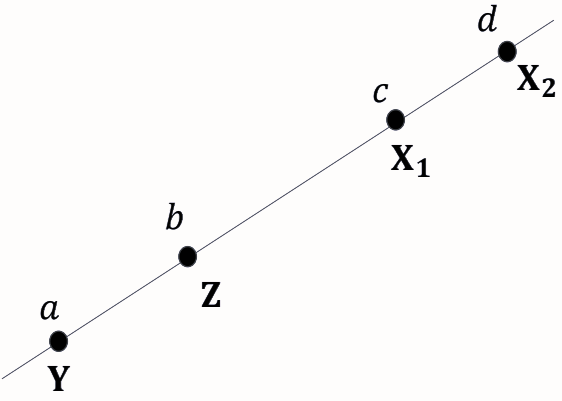
\includegraphics[width=0.25\linewidth]{images/line.png}
        \caption{Line with the point of previous problem}
    \end{figure}
    \begin{proof}
        Since the abscissae are proportional we can replace the abscissae by the $X$ coordinate like in the figure. 
        \begin{figure}[H]
            \centering
            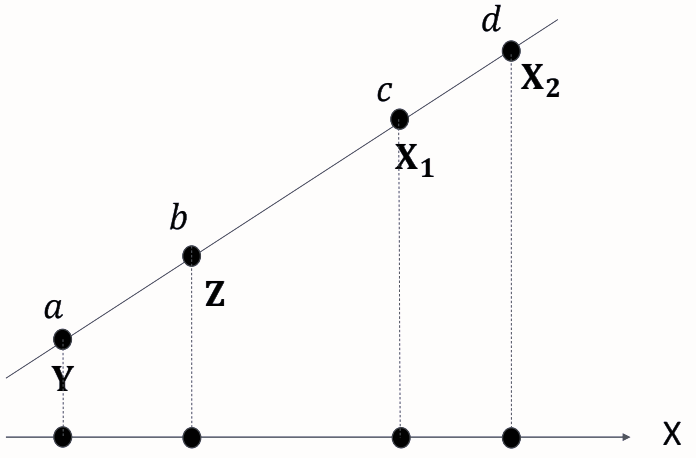
\includegraphics[width=0.4\linewidth]{images/abscissae.png}
        \end{figure}
        And the relation 
        \[CR_{X_1,X_2,Y,Z}=\dfrac{c-a}{c-b}/\dfrac{d-a}{d-b}\]
        still holds. Let $\textbf{Y}=\begin{bmatrix} y \\ * \\ v \end{bmatrix}$ and $\textbf{Z}=\begin{bmatrix} z \\ * \\ w \end{bmatrix}$, then: 
        \[ \textbf{X}_1=\begin{bmatrix} \alpha_1y+\beta_1z \\ * \\ \alpha_1v+\beta_1w \end{bmatrix} \:\:\:\:\:\:\:\:\:\:\:\:
        \textbf{X}_2=\begin{bmatrix} \alpha_2y+\beta_2z \\ * \\ \alpha_2v+\beta_2w \end{bmatrix}\]
        The difference between the $X$ coordinates of $\textbf{X}_1$ and $Y$ is:
        \[c-a=\dfrac{\beta_1(zv-yw)}{(\alpha_1y+\beta_1z)v}\]
        The difference between the $X$ coordinates of $\textbf{X}_1$ and $Z$ is:
        \[c-b=\dfrac{-\alpha_1(zv-yw)}{(\alpha_1y+\beta_1z)w}\]
        By substitution we obtain: 
        \[ \dfrac{c-a}{c-b}=-\dfrac{\beta_1w}{\alpha_1v} \:\:\:\:\:\:\:\:\:\:\:\: \dfrac{d-a}{d-b}=-\dfrac{\beta_2w}{\alpha_2v}\]
    \end{proof}

    \section{Conics}
    The conics derives from the intersection of cones with planes. 
    \begin{figure}[H]
        \centering
        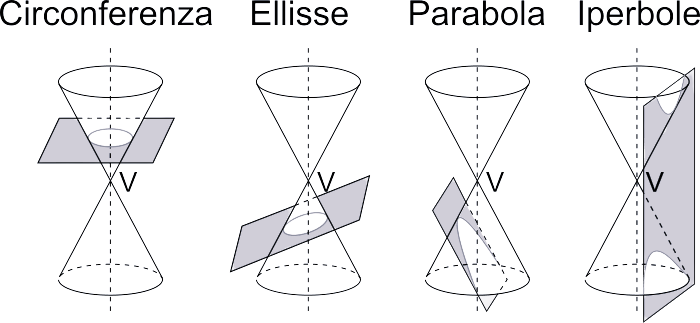
\includegraphics[width=0.75\linewidth]{images/conics.png}
        \caption{A circumference, an ellipse, a parabola and a hyperbole}
    \end{figure}
    \begin{definition}
        A point $\textbf{x}$ is on a \emph{conic} $\textbf{C}$ if it satisfies a homogeneous quadratic equation, namely
        \[\textbf{x}^T\textbf{C}\textbf{x}=0\]
        where $\textbf{C}$ is a symmetric matrix (this is a convention). 
    \end{definition}
    A conic is a curve described by a second-degree equation in the plane. In Euclidean coordinates a conic becomes: 
    \[aX^2+bXY+cY^2+dX+eY+f=0\]
    and in homogeneous coordinates becomes: 
    \[ax^2+bxy+cy^2+dxw+eyw+fw^2=0\]
    or in matrix form: 
    \[\textbf{x}^T \begin{bmatrix} a & b/2 & d/2 \\ b/2 & c & e/2 \\ d/2 & e/2 & f \end{bmatrix} \textbf{x}=0\]
    The conics have five degrees of freedom, so we need five points to define a unique conic. 
    \begin{example}
        The circumference can be expressed in Cartesian coordinates: 
        \[(X-X_0)^2+(Y-Y_0)^2-r^2=0\]
        or in homogeneous coordinates: 
        \[  \begin{bmatrix} x & y & w \end{bmatrix}
            \begin{bmatrix} 1 & 0 & -X_0 \\ 0 & 1 & -Y_0 \\ -X_0 & -Y_0 & X_0^2+Y_0^2-r^2 \end{bmatrix}
            \begin{bmatrix} x \\ y \\ w \end{bmatrix} = 0
        \]
    \end{example}
    Given a quadratic equation of a conic and a linear equation of a line, their intersection leads to a two degree equation on $\textbf{x}$. This means that there are always two 
    intersection points between a line and a conic, and they can be: real or complex conjugate and distinct or coincident. This result is due to the fundamental theorem of algebra. 
    \begin{theorem}[Fundamental theorem of algebra]
        The fundamental theorem of algebra states that every non-constant single-variable polynomial with complex coefficients has at least one complex root.
    \end{theorem}
    \begin{figure}[H]
        \centering
        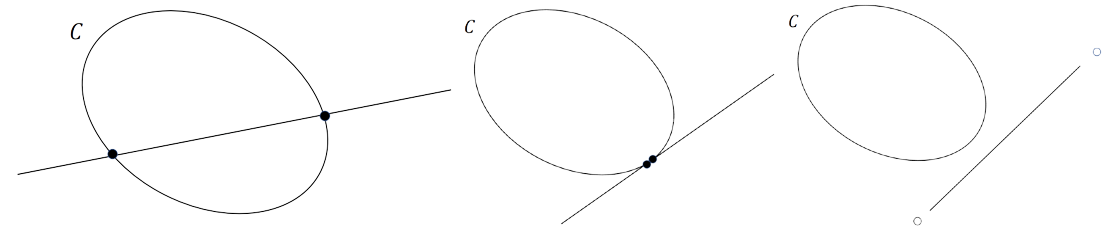
\includegraphics[width=0.75\linewidth]{images/intersection.png}
        \caption{Intersection with two real roots, two coincident roots and two imaginary roots}
    \end{figure}
    The intersection between the line at the infinity and a conic is:
    \begin{itemize}
        \item A parabola if there are two coincident solutions, that is the point at the infinity along axis.
        \item An ellipse if there are two complex-conjugate, that is there are no real solution. 
        \item A hyperbole if there are two real distinct solutions, that is the lines are the asymptotes.
    \end{itemize}

    \subsection{Circular points}
    \begin{example}
        Intersecting a circumference and the line at the infinity we obtain the following system: 
        \[\begin{cases}
            x^2-2X_0w+X_0^2w^2+y^2-2Y_0w+Y_0^2w^2-r^2w^2=0 \\
            w=0
        \end{cases}\]
        We obtain: 
        \[x^2+y^2=0\]
        As we can see, the circumference parameters (center and radius) disappear from the equation. So, we have that the two intersection points are the same for all circumferences. 
    \end{example}
    \begin{definition}
        The two intersection points are the same for all circumferences with the line at the infinity are the points: 
        \[\textbf{I}=\begin{bmatrix} 1 \\ i \\ 0 \end{bmatrix} \:\:\:\:\:\: \textbf{J}=\begin{bmatrix} 1 \\ -i \\ 0 \end{bmatrix}\]
        called \emph{circular points}. 
    \end{definition}

    \subsection{Polar line}
    \begin{definition}
        Given a point $\textbf{y}$ and a conic $\textbf{C}$ in the plane, the line $\textbf{l}=C\textbf{y}$ is called the \emph{polar line} of point $\textbf{y}$ with respect
        to the conic $\textbf{C}$. 
    \end{definition}
    \begin{figure}[H]
        \centering
        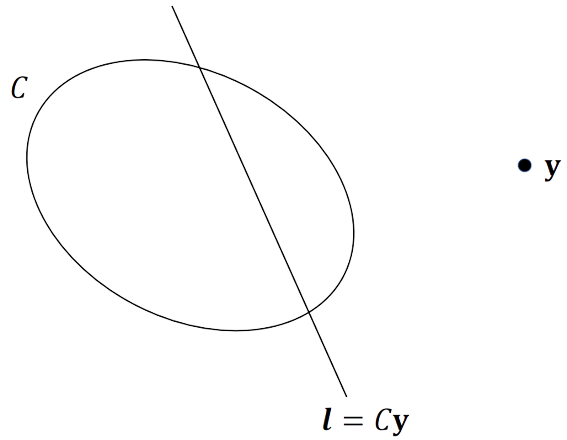
\includegraphics[width=0.5\linewidth]{images/polar.png}
        \caption{Example of polar line}
    \end{figure}
    
    \subsection{Harmonic tuples}
    \begin{definition}
        A 4-tuple of colinear points A, B, C, D, whose cross ratio is = -1, is said to be a \emph{harmonic tuple}. 
    \end{definition}
    This value, of course, is also assumed by the cross ratio of other 4-tuples of colinear points. A notable example is: 
    \[\left( T,Z,\textnormal{mid\_point}(Y,Z),P(\textnormal{at the infinity}) \right)\]
    If $(A, B, C, D)$ is a harmonic 4-tuple, also $(C, D, A, B)$ is harmonic. 
    \begin{definition}
        In a harmonic tuple $(A, B, C, D)$, $A$ and $B$ are said to be \emph{conjugate} of each other with respect to $C$ and $D$.
    \end{definition}
    Since the cross ratio of a harmonic tuple is negative, then two conjugate points $A, B$ with respect to $C, D$ are one inside segment $(C,D)$ and one outside $(C,D)$. 

    \subsection{Polar line and harmonic tuples}
    Consider any point $\textbf{z}$ on the polar line $\textbf{l}=C\textbf{y}$, and consider the line through $\textbf{y}$ and $\textbf{z}$: call $\textbf{x}_1$ and
    $\textbf{x}_2$ the points where this line crosses the conic. 
    \begin{figure}[H]
        \centering
        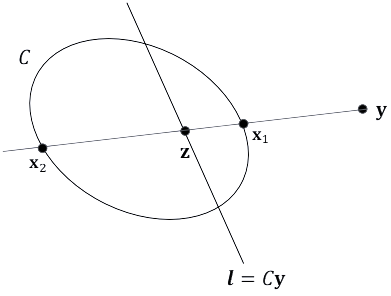
\includegraphics[width=0.5\linewidth]{images/polarharmonic.png}
    \end{figure}
    \begin{theorem}
        Let $\textbf{x}_1$ and $\textbf{x}_2$ be the points where the line through $\textbf{y}$ and $\textbf{z}$ crosses $C$: $\textbf{y}$ and $\textbf{z}$ are conjugate 
        with respect to $\textbf{x}_1$ and $\textbf{x}_2$.        
    \end{theorem}
    The polar line $\textbf{l}=C\textbf{y}$ is the locus of the points conjugate of $\textbf{y}$ with respect to conic $C$ (more precisely, conjugate with respect to the 
    intersection points of $C$ with any line through $\textbf{y}$). 

    \subsection{Polar line and tangency points}
    Since $\textbf{y}$ is outside segment ($\textbf{x}_1$,$\textbf{x}_2$) then its conjugate $\textbf{z}$ is inside ($\textbf{x}_1$,$\textbf{x}_2$). This holds for any 
    line through $\textbf{y}$. As the line through $\textbf{y}$ tends to be tangent to $C$, the points $\textbf{x}_1$ and $\textbf{x}_2$ coincide with the tangency point to 
    $C$ : therefore the conjugate point $\textbf{z}$, which remains inside ($\textbf{x}_1$,$\textbf{x}_2$), is also coincident with the tangency point. The conjugate point 
    $\textbf{z}$, which remains inside ($\textbf{x}_1$,$\textbf{x}_2$), also coincides with the tangency point. Analogous result holds for the other line tangent to $C$ from 
    $\textbf{y}$. 

    So, we have obtained that the polar line $\textbf{l}=C\textbf{y}$ goes through the tangency points from $\textbf{y}$ to $C$.  

    We have that points $\textbf{z}$ and $\textbf{y}$ are conjugate with respect to the conic $C$. So, if point $\textbf{z}$ is on the conic $C$, then point $\textbf{y}$ 
    is one of its conjugates. We have that the tangent line $\textbf{l}_{\textbf{z}}$ to $C$ through $\textbf{z}$ is the locus of points conjugate to $\textbf{z}$. So, we 
    have that $\textbf{l}_{\textbf{z}}$ is the polar line of $\textbf{z}$ with respect to $C$. 
    \begin{figure}[H]
        \centering
        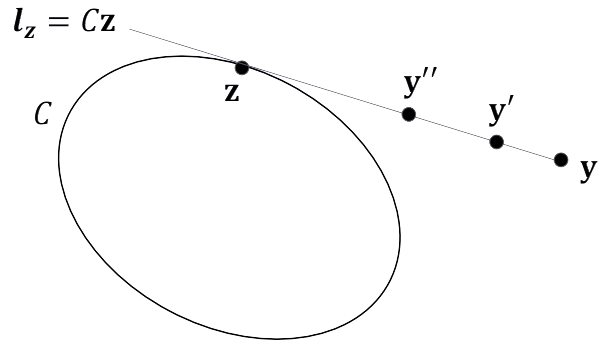
\includegraphics[width=0.5\linewidth]{images/tangentpolar.png}
    \end{figure}
    We can see that the polar line $\textbf{l}_{\textbf{z}}=C\textbf{z}$ of a point $\textbf{z}$ on the conic $C$ is the tangent line to $C$ through $\textbf{z}$. 
    \begin{example}
        Consider a circumference with radius $r$ centered in the origin of the plane and the point $\textbf{y}={\begin{bmatrix} X & 0 & 1 \end{bmatrix}}^T$, its equation is: 
        \[
        \textbf{l}=C\textbf{y}=
        \begin{bmatrix}
            1 & 0 & 0 \\
            0 & 1 & 0 \\
            0 & 0 & -r^2
        \end{bmatrix}    
        \begin{bmatrix}
            X \\
            0 \\
            1 
        \end{bmatrix}    
        = 
        \begin{bmatrix}
            X \\
            0 \\
            -r^2 
        \end{bmatrix}  
        \]
        So we obtained that the polar line has the following Cartesian equation: 
        \[X x-r^2 = 0 \rightarrow x=\dfrac{r^2}{X}\]
        that is a vertical line. 
    \end{example}
    With the previous example we obtained that the polar of a point $P$ with respect to a circumference is a line perpendicular to the segment $(\textnormal{center}, P)$. 
    \begin{example}
        Consider a circumference with radius $r$ centered in the origin of the plane and the point $\textbf{y}={\begin{bmatrix} x & 0 & 0 \end{bmatrix}}^T$, its equation is: 
        \[
        \textbf{l}=C\textbf{y}=
        \begin{bmatrix}
            1 & 0 & 0 \\
            0 & 1 & 0 \\
            0 & 0 & -r^2
        \end{bmatrix}    
        \begin{bmatrix}
            x \\
            0 \\
            0 
        \end{bmatrix}    
        = 
        \begin{bmatrix}
            X \\
            0 \\
            0 
        \end{bmatrix}  
        \]
        So we obtained that the polar line has the following Cartesian equation: 
        \[X x=0 \rightarrow X=0\]
        that is at the diameter of the circumference perpendicular at the direction of the point $\textbf{y}$. 
    \end{example}
    Tangent lines from a point at the infinity are all parallel, so we have that tangency points are along a diameter perpendicular to the common direction of the parallel tangents. 
    \begin{figure}[H]
        \centering
        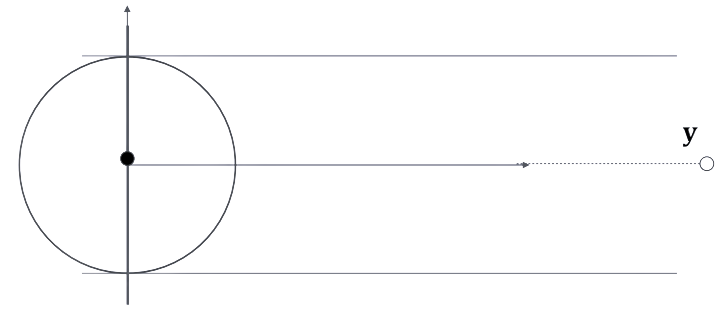
\includegraphics[width=0.5\linewidth]{images/parallel.png}
    \end{figure}
    \begin{example}
        Consider a circumference with radius $r$ centered in the origin of the plane and the point $\textbf{y}={\begin{bmatrix} x & 0 & 0 \end{bmatrix}}^T$, its equation is: 
        \[
        \textbf{l}=C\textbf{y}=
        \begin{bmatrix}
            1 & 0 & 0 \\
            0 & 1 & 0 \\
            0 & 0 & -r^2
        \end{bmatrix}    
        \begin{bmatrix}
            0 \\
            0 \\
            1 
        \end{bmatrix}    
        = 
        \begin{bmatrix}
            0 \\
            0 \\
            -r^2 
        \end{bmatrix}  
        \]
        So we obtained that the polar line has the following Cartesian equation: 
        \[-r^2w=0 \rightarrow X=0\]
        that is at the line at the infinity. 
    \end{example}
    In general, we have the following properties: 
    \begin{enumerate}
        \item The polar line of any point at the infinity is a diameter.
        \item Any diameter goes through the center of the circumference.
        \item The center is conjugate to each point at the infinity.
        \item All the points at the infinity are conjugate to the center.
        \item The polar of the center is the line containing all the points at the infinity.
        \item The polar line of the center is the line at the infinity.
    \end{enumerate}

    \subsection{Degenerate conics}
    \begin{definition}
        A \emph{non-degenerate conic} is a conic where the matrix $\textbf{C}$ is non-singular: 
        \[\textnormal{rank}(\textbf{C})=3\]

        A \emph{degenerate conic} is a conic where the matrix $\textbf{C}$ is singular: 
        \[\textnormal{rank}(\textbf{C}) < 3\]
    \end{definition}
    There are two possible cases: 
    \begin{itemize}
        \item $\textnormal{rank}(\textbf{C}) = 2$: in this case any symmetric $3 \times 3$ matrix $\textbf{C}$ can be written as:
            \[\textbf{C}=\textbf{lm}^T+\textbf{ml}^T\]
            where $\textbf{l}$ and $\textbf{m}$ are column vectors. This conic is the set of points $\textbf{x}$ satisfying $\textbf{x}^T\textbf{C}\textbf{x}=0$. This equation is 
            satisfied if $\textbf{x}^T\textbf{l}=\textbf{0}$ or $\textbf{m}^T\textbf{x}=\textbf{0}$ are satisfied. So, we have that $\textbf{x}$ is on the set union of lines 
            $\textbf{l}$ and $\textbf{m}$.
            \begin{figure}[H]
                \centering
                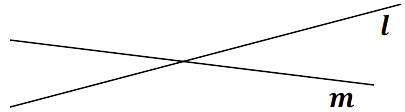
\includegraphics[width=0.5\linewidth]{images/inters.png}
            \end{figure}
        \item $\textnormal{rank}(\textbf{C}) = 1$: in this case any symmetric $3 \times 3$ matrix $\textbf{C}$ can be written as:
            \[\textbf{C}=\textbf{ll}^T\]
            where $\textbf{l}$ is a column vector. This conic is the set of points $\textbf{x}$ satisfying $\textbf{x}^T\textbf{C}\textbf{x}=0$. This equation is 
            satisfied if $\textbf{x}^T\textbf{l}=\textbf{0}$ is satisfied (counted two times). So, we have that $\textbf{x}$ is on the repeated line $\textbf{l}$. 
            \begin{figure}[H]
                \centering
                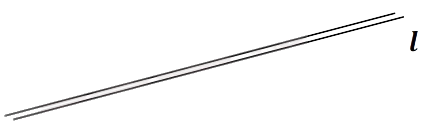
\includegraphics[width=0.5\linewidth]{images/rep.png}
            \end{figure}
    \end{itemize}

    \section{Dual conics}
    \subsection{Definition}
    \begin{definition}
        A \emph{dual conic} is a set of lines $\textbf{l}$ that satisfy equation
        \[\textbf{l}^T\textbf{C}^{*}\textbf{l}=\textbf{0}\]
        where $\textbf{C}^{*}$ is a $3 \times 3$ symmetric matrix.

        A \emph{non-degenerate dual conic} is a dual conic whose matrix $\textbf{C}^{*}$ is non-singular: 
        \[\textnormal{rank}(\textbf{C}^{*})=3\]
    \end{definition}
    Consider a non-degenerate conic $\textbf{C}$ and the set of all lines $\textbf{l}$ that are tangent to it: through each point $\textbf{c}$ on $\textbf{C}$ there is a line 
    $\textbf{l}$ tangent to $\textbf{C}$. Since $\textbf{l}$ is the polar of $\textbf{x}$ with respect to $\textbf{C}$, is $\textbf{l}=\textbf{Cc}$. Therefore, is
    \[\textbf{x}=\textbf{C}^{-1}\textbf{l}\]
    and hence, since $\textbf{C}$ is symmetric we have 
    \[\textbf{x}^T=\textbf{l}^T\textbf{l}^{-T}=\textbf{l}^T\textbf{C}^{-1}\]
    Now, since the point $\textbf{x}$ is on $\textbf{C}$,
    \[\textbf{x}^T\textbf{C}\textbf{x}=\textbf{0}\]
    Substituting the values found previously we obtain: 
    \[\textbf{l}^T\textbf{C}^{-1}\textbf{l}=\textbf{0}\]
    that is the quadratic homogeneous equation on $\textbf{l}$. So we can say that for the dual conic $\textbf{C}^{*}=\textbf{C}^{-1}$

    We can also say that a non-degenerate dual conic $\textbf{C}^{*}$ is the set of lines tangent to a non-degenerate conic $\textbf{C}$. 

    \subsection{Degenerate dual conics}
    \begin{definition}
        A \emph{degenerate dual conic} is a conic where the matrix $\textbf{C}^{*}$ is singular: \[\textnormal{rank}(\textbf{C}^{*}) < 3\]
    \end{definition}
    There are two possible cases: 
    \begin{itemize}
        \item $\textnormal{rank}(\textbf{C}^{*}) = 2$: in this case any symmetric $3 \times 3$ matrix $\textbf{C}^{*}$ can be written as:
            \[\textbf{C}^{*}=\textbf{pq}^T+\textbf{qp}^T\]
            This conic is the line $\textbf{l}$ going through point \textbf{p} or the line $\textbf{l}$ going through point \textbf{q}. 
            \begin{figure}[H]
                \centering
                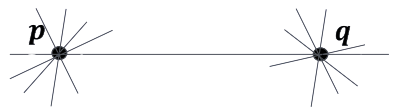
\includegraphics[width=0.5\linewidth]{images/deg2.png}
            \end{figure}
        \item $\textnormal{rank}(\textbf{C}^{*}) = 1$: in this case any symmetric $3 \times 3$ matrix $\textbf{C}^{*}$ can be written as:
            \[\textbf{C}^{*}=\textbf{pp}^T\]
            This conic is the line $\textbf{l}$ going through point \textbf{p} repeated twice. 
            \begin{figure}[H]
                \centering
                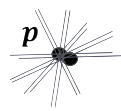
\includegraphics[width=0.2\linewidth]{images/deg1.png}
            \end{figure}
    \end{itemize}

    \begin{definition}
        The degenerate dual conic $\textbf{C}^{*}=\textbf{pq}^T+\textbf{qp}^T$ going through two circular point $\textbf{p}$ and $\textbf{q}$ is called the conic dual to the 
        circular points, and it is equal to: 
        \[\textbf{C}^{*}_{\infty}=\textbf{IJ}^{T}+\textbf{JI}^{T}=
        \begin{bmatrix}
            1 & 0 & 0 \\
            0 & 1 & 0 \\
            0 & 0 & 0 
        \end{bmatrix}\]
    \end{definition}

    \section{Transformations}
    \begin{definition}
        A \emph{projective mapping} between a projective plane $\mathbb{P}^2$ and another projective plane $\mathbb{P}^{'2}$ is an invertible mapping which preserves colinearity:
        \[h:\mathbb{P}^2 \rightarrow \mathbb{P}^{'2}, \textbf{x}^{'}=h(\textbf{x}),\textbf{x}_1,\textbf{x}_2,\textbf{x}_3 \textnormal{ are colinear}\]
        \[\Leftrightarrow\]
        \[\textbf{x}_1^{'}=h(\textbf{x}_1),\textbf{x}_2^{'}=h(\textbf{x}_2),\textbf{x}_3^{'}=h(\textbf{x}_3) \textnormal{ are colinear}\]
    \end{definition}
    Projective mapping is also called projectivity or homography. 
    \begin{example}
        Mappings between two planes induced by central projection are projective, since they preserve colinearity. 
        \begin{figure}[H]
            \centering
            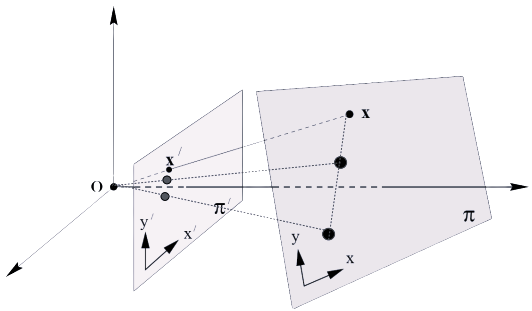
\includegraphics[width=0.5\linewidth]{images/map1.png}
        \end{figure}
        Mapping between a planar scene and its image is a homography, since it is induced by a central projection
        \begin{figure}[H]
            \centering
            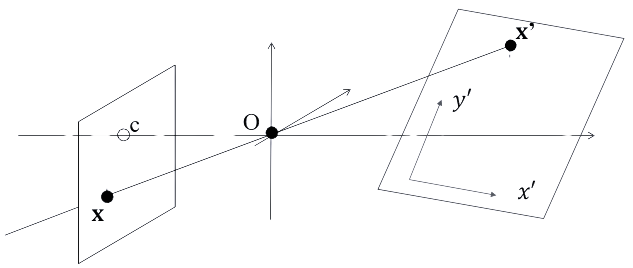
\includegraphics[width=0.5\linewidth]{images/map2.png}
        \end{figure}
        Mapping between two images of a planar scene is a homography.
        \begin{figure}[H]
            \centering
            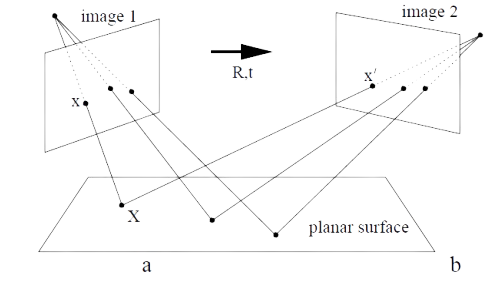
\includegraphics[width=0.5\linewidth]{images/map3.png}
        \end{figure}
        Two images of a 3D scene, taken by a camera rotating around its center are related by a homography, since the second image is a central projection of the first image. 
        \begin{figure}[H]
            \centering
            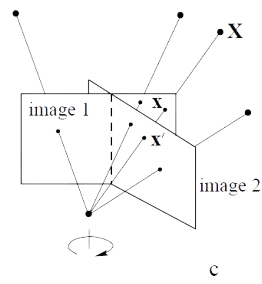
\includegraphics[width=0.4\linewidth]{images/map4.png}
        \end{figure}
        The shadow cast by a planar silhouette onto a ground plane is a projective transformation of the planar silhouette, since they are related by a central projection. 
        \begin{figure}[H]
            \centering
            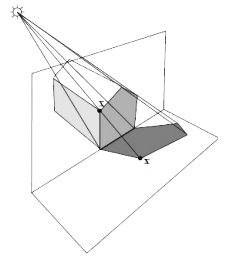
\includegraphics[width=0.3\linewidth]{images/map5.png}
        \end{figure}
    \end{example}
    \begin{theorem}[Fundamental theorem of projective geometry]
        A mapping $h:\mathbb{P}^{2} \rightarrow \mathbb{P}^{'2}$ is projective if and only if there exists an invertible $3 \times 3$ matrix $H$ such that for any point in 
        $\mathbb{P}^{2}$ represented by the vector $\mathbf{x}$, is $h(\textbf{x})=H\textbf{x}$, where: 
        \[H=\begin{bmatrix}
            h_{11} & h_{12} & h{13} \\
            h_{21} & h_{22} & h{23} \\
            h_{31} & h_{32} & h{33} 
        \end{bmatrix}\]
    \end{theorem}
    Projective mappings are linear in the homogeneous coordinates, but they are not in Cartesian coordinates. 

    From the theorem we have that $h(\textbf{x})=\textbf{x}^{'}=H\textbf{x}$. Therefore, if we multiply the matrix $H$ by any nonzero scalar $\lambda$, the relation is satisfied by 
    the same points $\textbf{x}^{'}=\lambda H\textbf{x}$. Thus, any nonzero multiple of the matrix $H$ represents the same projective mapping as $H$. Hence, $H$ is a homogeneous 
    matrix: in spite of its $9$ entries, $H$ has only $8$ degrees of freedom, namely the ratios between its elements. Therefore, it can be estimated by just four point 
    correspondences, since each point correspondence $\textbf{x}^{'}=H\textbf{x}$ yields two independent equations. 

    \begin{definition}
        A homography transform each: 
        \begin{enumerate}
            \item Point $\textbf{x}$ into a point $\textbf{x}^{'}$ such that: $\textbf{x} \rightarrow H \textbf{x}=\textbf{x}^{'}$
            \item Line $\textbf{l}$ into a line $\textbf{l}^{'}$ such that: $\textbf{l} \rightarrow H^{-T} \textbf{l}=\textbf{l}^{'}$
            \item Conic $C$ into a conic $C^{'}$ such that: $C \rightarrow H^{-T} CH^{-1}=C^{'}$
            \item Dual conic $C^{*}$ into a dual conic $C^{*'}$ such that: $C^{*} \rightarrow H C^{*}H^{T}=C^{*'}$
        \end{enumerate}
    \end{definition}
    \begin{proof}[property two]
        The equation of the line on $\textbf{x}$ is $\textbf{l}^T\textbf{x}=\textbf{0}$ has to be converted into a constraint on $\textbf{x}^{'} = H \textbf{x}$. Combining the two 
        equations we obtain a linear equation on $\textbf{x}^{'}$: 
        \[\textbf{l}^{'T}\textbf{x}^{'}=\textbf{0}\]
        With $\textbf{l}^{'T}=\textbf{l}^{T}H^{-1}$ and so we have: 
        \[\textbf{l}^{'}=H^{-T}\textbf{l}\]
    \end{proof}
    \begin{proof}[property three]
        The equation of the conic on $\textbf{x}$ is $\textbf{x}^{T}\textbf{C}\textbf{x}=\textbf{0}$ has to be converted into a constraint on $\textbf{x}^{'} = H \textbf{x}$, that 
        is equal to:
        \[\textbf{x}=H^{-1}\textbf{x}^{'} \textnormal{ and } \textbf{x}^{T}=\textbf{x}^{iT}H^{-T}\]
        Combining the three equations we obtain a linear equation on $\textbf{x}^{'}$: 
        \[\textbf{x}^{'T}\textbf{C}^{'}\textbf{x}^{'}=\textbf{0}\]
        And so we have: 
        \[C^{'}=H^{-T} CH^{-1}\]
    \end{proof}
    \begin{proof}[property four]
        It is possible to apply the same idea to prove the transformation of a dual conic, obtaining:
        \[C^{*'}=H C^{*}H^{T}\]
    \end{proof}
    The point line incidence is preserved. 
    \begin{proof}
        Suppose that point $\textbf{x}$ is on the line $\textbf{l}$, that is $\textbf{l}^T\textbf{x}=\textbf{0}$. Apply the same projective transformation $H$ both to $\textbf{x}$ 
        and $\textbf{l}$: $H\textbf{x}=\textbf{x}^{'}$ and $H^{-1}\textbf{l}=\textbf{l}^{'}$. They are still incident if $\textbf{l}^{'T}\textbf{x}^{'}=\textbf{0}$:
        \[\textbf{l}^{'T}\textbf{x}^{'}=\textbf{l}^{T}H^{-1}\textbf{x}^{'}=\textbf{l}^{T}H^{-1}H\textbf{x}=\textbf{l}^{T}\textbf{x}=\textbf{0}\]
    \end{proof}

    \subsection{Vanishing points and vanishing line}
    The point common to both parallel lines $\textbf{l}_1={\begin{bmatrix} a & b & c_1 \end{bmatrix}}^{T}$ and $\textbf{l}_2={\begin{bmatrix} a & b & c_2 \end{bmatrix}}^{T}$ is the 
    point $\textbf{x}={\begin{bmatrix} b & -a & 0 \end{bmatrix}}^{T}$, that is the point at the infinty along the direction of both lines. If we search for the common point of 
    infinte lines $\textbf{l}_i$ we obtain that thay all have in common the point: 
    \[\textbf{x}_{\infty}={\begin{bmatrix} b & -a & 0 \end{bmatrix}}^{T}\]
    So, we obtained that all lines are concurrent at ${\begin{bmatrix} b & -a & 0 \end{bmatrix}}^{T}$. 
    
    Applying a projective transformation to all the above parallel lines $\textbf{l}_i$ we obtain lines $\textbf{l}_i^{'}$. The common point $\textbf{x}_{\infty}$ to all lines
    $\textbf{l}_i$ is mapped onto a point $\textbf{x}_{\infty}^{'}$ which belongs to each of the lines $\textbf{l}_i^{'}$. 
    \begin{figure}[H]
        \centering
        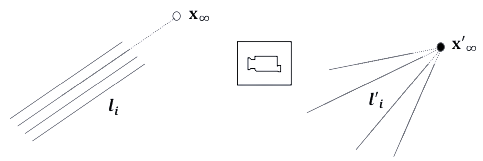
\includegraphics[width=0.5\linewidth]{images/vanishing.png}
    \end{figure}
    So, we have that all lines $\textbf{l}_i^{'}$ are concurrent at the point $\textbf{x}_{\infty}^{'}=H\textbf{x}_{\infty}$ called the vanishing point associated to the direction 
    $(b,-a)$, of the parallel lines. 
    \begin{theorem}
        The image of a set of parallel lines $\textbf{l}_i$ is a set of lines $\textbf{l}_i^{'}$ concurrent at a common point $\textbf{x}^{'}$ called the vanishing point of the 
        direction of lines $\textbf{l}_i$. 
    \end{theorem}

    Applying a projective transformation to line at the infinity $\textbf{l}_{\infty}$ we obtain a line $\textbf{l}_{\infty}^{'}$. This line goes through the image all the points at 
    the infinity $\textbf{x}_{\infty}$ of the original plane. So, we have that the vanishing line $\textbf{l}_{\infty}^{'}$ can be determined from two vanishing points. 
    \begin{figure}[H]
        \centering
        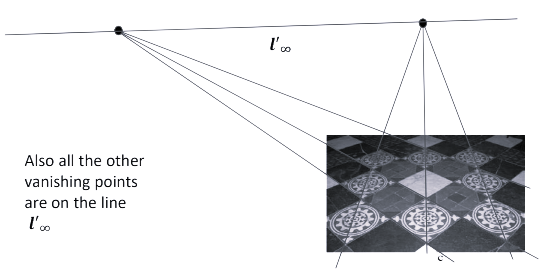
\includegraphics[width=0.75\linewidth]{images/vanishingline.png}
    \end{figure}

    \subsection{Polarity}
    Polarity is preserved under projective mappings. The polar line $\textbf{l}=\textbf{Cx}$ of a point $\textbf{x}$ with respect to a conic $\textbf{C}$ is mapped onto the polar line 
    of the transformed point $\textbf{x}^{'}=H\textbf{x}$ with respect to the transformed conic: 
    \[\textbf{C}^{'}=H^{-T}\textbf{C}H^{-1}\]
    \begin{proof}
        This property is satisfied because we have: 
        \[\textbf{C}^{'}\textbf{x}^{'}=H^{-T}\textbf{C}H^{-1}H\textbf{x}=H^{-T}\textbf{Cx}=H^{-T}\textbf{l}=\textbf{l}^{'}\]
    \end{proof}
    \begin{figure}[H]
        \centering
        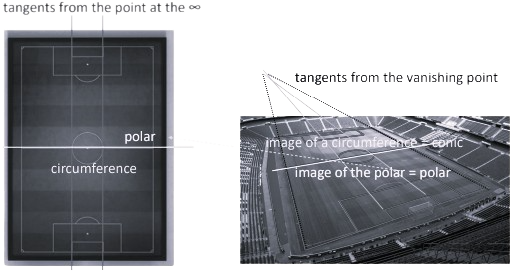
\includegraphics[width=0.75\linewidth]{images/polarity.png}
    \end{figure}
    In the end we have that since polarity is preserved, also conjugacy is preserved under projective mappings and also $CR=-1$ is preserved.

    \subsection{Cross ratio}
    Given a line with four points that have the following relations: 
    \[\textbf{X}_1=\propto_1\textbf{Y}+\beta_1\textbf{Z}\]
    \[\textbf{X}_2=\propto_2\textbf{Y}+\beta_2\textbf{Z}\]
    We have that the cross ratio is the following: 
    \[CR_{X_1,X_2,Y,Z}=\dfrac{\beta_1/\alpha_1}{\beta_2/\alpha_2}\]
    If we apply a projective transformation $H$ to the four points we will have: 
    \[\textbf{Y}^{'}=\textbf{HY} \:\:\:\:\:\: \textbf{Z}^{'}=\textbf{HZ}\] 
    \[\textbf{X}^{'}_1=\textbf{HX}_1=\textbf{X}_1=\propto_1\textbf{Y}^{'}+\beta_1\textbf{Z}^{'} \:\:\:\:\:\: \textbf{X}^{'}_2=\textbf{HX}_2=\propto_2\textbf{Y}^{'}+\beta_2\textbf{Z}^{'}\]
    The linear combination coefficients are the same. Therefore their cross ratio is preserved and it is again: 
    \[CR_{X_1^{'},X_2^{'},Y^{'},Z^{'}}=\dfrac{\beta_1/\alpha_1}{\beta_2/\alpha_2}=CR_{X_1,X_2,Y,Z}\]

    \subsection{Hierarchy of projective transformations}
    \begin{figure}[H]
        \centering
        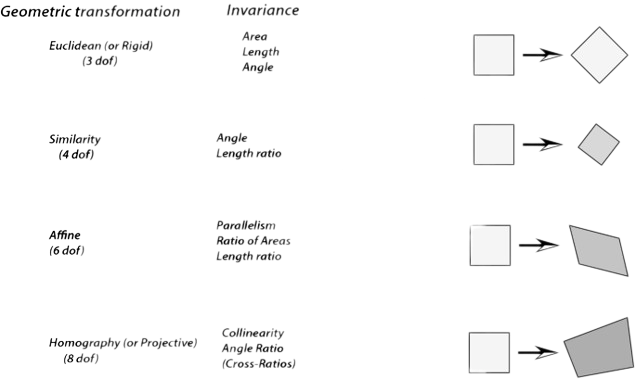
\includegraphics[width=1\linewidth]{images/hierarchy.png}
    \end{figure}

    \subsection{Isometries}
    The isometries have three degree of freedom, which are the translation $\textbf{t}$ and the rotation angle $\vartheta$. So, the invariants of this transformation are: lengths, 
    distances, and areas. 
    \begin{figure}[H]
        \centering
        
\includegraphics[width=0.5\linewidth]{images/isometry.png}
    \end{figure}
    \begin{definition}
        The orthogonal matrix $R_{\perp}$ is defined as follows: 
        \[R_{\perp}^{-1}=R_{\perp}^{T}\]
    \end{definition}
    So, we have that the matrix $H_I$ for the isometries is the follow: 
    \[H_I=
    \begin{bmatrix}
        \cos \vartheta & -\sin \vartheta & t_x \\
        \sin \vartheta & \cos \vartheta & t_y \\
        0 & 0 & 1
    \end{bmatrix}\]
    Where $
    \begin{bmatrix}
        \cos \vartheta & -\sin \vartheta \\
        \sin \vartheta & \cos \vartheta
    \end{bmatrix}
    =R_{\perp}$
    \begin{figure}[H]
        \centering
        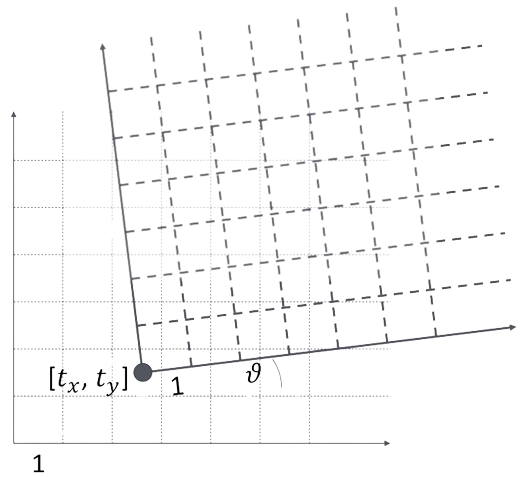
\includegraphics[width=0.5\linewidth]{images/isometry1.png}
    \end{figure}

    \subsection{Similarities}
    The similarities have four degree of freedom, which are the translation $\textbf{t}$, the scale $s$, and the rotation angle $\vartheta$. So, the invariants of this transformation are: ratio of lenghts, and angles.
    Also, the circular points $\textbf{I}$ and $\textbf{J}$ are invariant of the transofrmation. 
    \begin{figure}[H]
        \centering
        
\includegraphics[width=0.5\linewidth]{images/similarity.png}
    \end{figure}
    So, we have that the matrix $H_S$ for the similarities is the follow: 
    \[H_I=
    \begin{bmatrix}
        s\cos \vartheta & -s\sin \vartheta & t_x \\
        s\sin \vartheta & s\cos \vartheta & t_y \\
        0 & 0 & 1
    \end{bmatrix}\]
    Where $
    \begin{bmatrix}
        s\cos \vartheta & -s\sin \vartheta \\
        s\sin \vartheta & s\cos \vartheta
    \end{bmatrix}
    =sR_{\perp}$
    \begin{figure}[H]
        \centering
        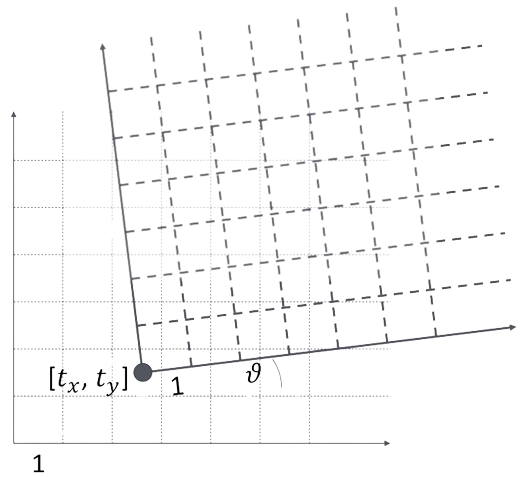
\includegraphics[width=0.5\linewidth]{images/isometry1.png}
    \end{figure}

    \subsection{Affinities}
    The affinities have six degree of freedom, which are the submatrix $A$ and the translation. So, the invariants of this transformation are: parallelism, ratio of parallel lenghts, ratio of areas.
    $A$ is any $2 \times 2$ (rank two) matrix. Also the line at the infinity $\textbf{l}_{\infty}$ is invariant of the transofrmation.
    \begin{figure}[H]
        \centering
        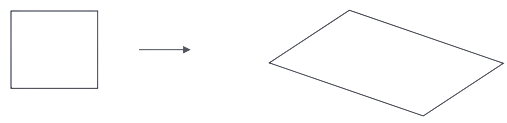
\includegraphics[width=0.5\linewidth]{images/affinities.png}
    \end{figure}
    So, we have that the matrix $H_A$ for the affinities is the follow: 
    \[H_I=
    \begin{bmatrix}
        a_{11} & a_{21} & t_x \\
        a_{12} & a_{21} & t_y \\
        0 & 0 & 1
    \end{bmatrix}\]
    Where $
    \begin{bmatrix}
        a_{11} & a_{21} \\
        a_{12} & a_{21} \\
    \end{bmatrix}
    =A$
    \begin{figure}[H]
        \centering
        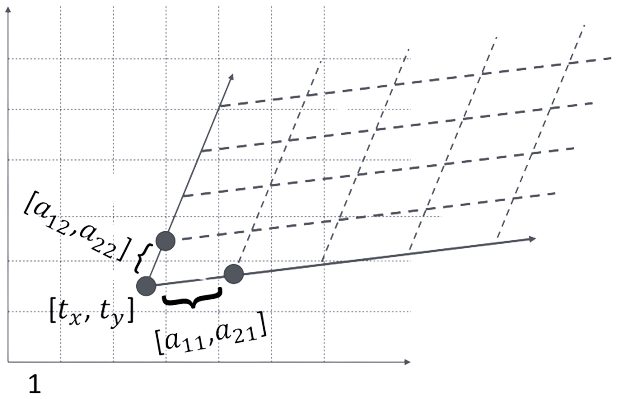
\includegraphics[width=0.5\linewidth]{images/affinities1.png}
    \end{figure}

    \subsection{Projectivities}
    The projectivities have eight degree of freedom, which are the sub-matrix $A$, the vector $v$, and the translation. So, the invariants of this transformation are: colinearity, incidence, order of contact.
    $A$ is any $2 \times 2$ (rank two) matrix. Also, the cross ratio is invariant of the transformation.
    \begin{figure}[H]
        \centering
        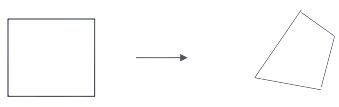
\includegraphics[width=0.5\linewidth]{images/projectivities.png}
    \end{figure}
    So, we have that the matrix $H_A$ for the projectivities is the follow: 
    \[H_I=
    \begin{bmatrix}
        a_{11} & a_{21} & t_x \\
        a_{12} & a_{21} & t_y \\
        v_1 & v_2 & 1
    \end{bmatrix}\]
    Where $
    \begin{bmatrix}
        a_{11} & a_{21} \\
        a_{12} & a_{21} \\
    \end{bmatrix}
    =A$
    \begin{figure}[H]
        \centering
        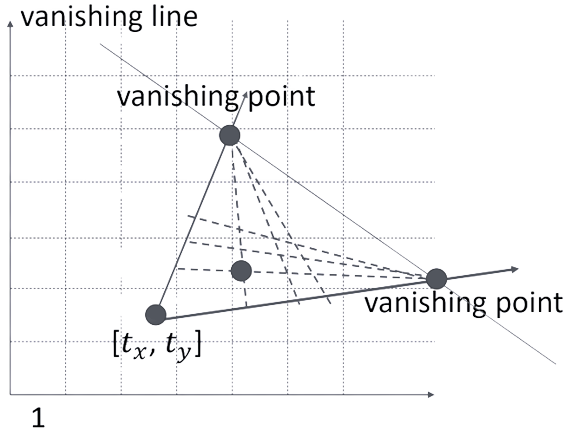
\includegraphics[width=0.5\linewidth]{images/projectivities1.png}
    \end{figure}

\newpage

\chapter{Two-dimensional reconstruction}
    \section{Introduction}
    We want to recover a model of the scene, given an image of an unknown planar scene. The scene is a set of unknown points $x_i$ on  a 
    plane. The image is a projective transformation of the scene, that is $\boldsymbol{x}_i^{'}=H\boldsymbol{x}_i$. In this equation we
    know only the $\boldsymbol{x}_i$ and not the matrix $H$. So, the main problem is that we cannot simply invert the 
    mapping $H$. 

    The general problem is unsolvable because we have too many unknowns. So, to find the projection matrix we can combine two strategies: 
    \begin{enumerate}
        \item Reduce unknowns: it is often not necessary to recover the original scene as it was, but it is simpler to recover just 
            the shape of the scene. In this case the goal is to recover a model similar to the scene, that is called shape reconstruction. 
            In this case, we can reduce the unknowns from eight to four and the matrix $H$ becomes: 
            \[H=    
            \begin{bmatrix}
                s\cos \vartheta & -s\sin \vartheta & t_x \\
                s\sin \vartheta & s\cos \vartheta & t_y \\
                0 & 0 & 1
            \end{bmatrix}\]
            We can also make a similarity instead of the shape, but this will reduce the unknowns only by two. The affinity will reduce
            the unknowns by six. 
        \item Add constraints: we use additional information to recover a model of the scene. The useful information is the values of
            parameters, that are invariant under the desired class of mappings, but are not invariant under more general classes. 
    \end{enumerate}

    \section{Reconstruction}
    The reconstruction can be of two types: 
    \begin{itemize}
        \item Affine reconstruction: reconstructed scene is an affine mapping of the original one. 
        \item Shape reconstruction: reconstructed scene is a similarity mapping of the original one. 
    \end{itemize}

    \subsection{Affine reconstruction}
    \begin{theorem}
        A projective transformation $H$ maps the line at the infinity $\boldsymbol{l}_{\infty}$ onto itself implies that and implies from $H$ is affine. 
    \end{theorem}
    \begin{proof}
        Any point at the infinity $\boldsymbol{x}_{\infty}=\begin{bmatrix} x \\ y \\ 0 \end{bmatrix}$ mapped onto a point 
        $\boldsymbol{x}^{'}=H\boldsymbol{x}_{\infty}$ also at the infinity if and only if the third coordinate of $\boldsymbol{x}^{'}$ is 
        zero. For all $(x,y)$ we have that 
        \[\begin{bmatrix} v_1 & v_2 & 1 \end{bmatrix} \begin{bmatrix} x \\ y \\ 0 \end{bmatrix}=0 \rightarrow \begin{bmatrix} v_1 & v_2 & 1 \end{bmatrix} = \begin{bmatrix} 0 & 0 & 1 \end{bmatrix}\]
        Namely, $H$ is affine.
    \end{proof}
    The given image is a general projective mapping of the original scene. This implies that the vanishing line $\boldsymbol{l}^{'}_{\infty}$
    is in general different from  $\boldsymbol{l}_{\infty}$. So, it is possible to use $\boldsymbol{l}^{'}_{\infty}$ as additional 
    information: if we apply to the image a new projective mapping $H_{AR}$ which sends $\boldsymbol{l}^{'}_{\infty}$ back to 
    $\boldsymbol{l}_{\infty}$, we obtain a new, modified image. The (new) image of the line at the infinity $\boldsymbol{l}_{\infty}$ is 
    again $\boldsymbol{l}_{\infty}$. 

    From the theorem, the obtained model (i.e. the new image) is an affine mapping of the original scene. So, the obtained model is an 
    affine reconstruction of the scene. 
    \begin{figure}[H]
        \centering
        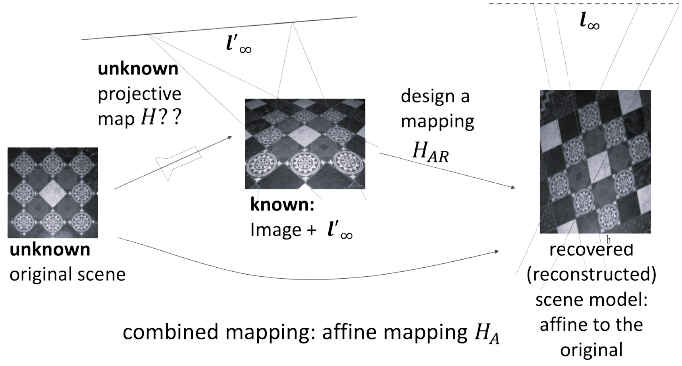
\includegraphics[width=0.75\linewidth]{images/HAR.png}
    \end{figure}
    The issues with this method are: 
    \begin{itemize}
        \item Find a projective mapping $H_{AR}$ which sends $\boldsymbol{l}^{'}_{\infty}$ back to $\boldsymbol{l}_{\infty}$: this mapping 
            must map any point $\boldsymbol{x}^{'} \in \boldsymbol{l}^{'}_{\infty}$ onto a set of point at the infinity: 
            \[H_{AR}\boldsymbol{x}^{'} = \begin{bmatrix} * \\ * \\ 0 \end{bmatrix}\]
            Everything works if we let \[H_{AR}=
            \begin{bmatrix}
                * & * & * \\
                * & * & * \\
                \: & \boldsymbol{l}^{'T}_{\infty} & \:
            \end{bmatrix}\]
            In fact we have: 
            \[H_{AR}\boldsymbol{x}^{'}=
            \begin{bmatrix}
                * & * & * \\
                * & * & * \\
                \: & \boldsymbol{l}^{'T}_{\infty} & \:
            \end{bmatrix}
            \boldsymbol{x}^{'}
            =
            \begin{bmatrix}
                * \\
                * \\
                \boldsymbol{l}^{'T}_{\infty}\boldsymbol{x}^{'}
            \end{bmatrix}
            \]
        \item Find the vanishing line: it is possible to use additional knowledge items, such as the image of parallel lines. 
            \begin{figure}[H]
                \centering
                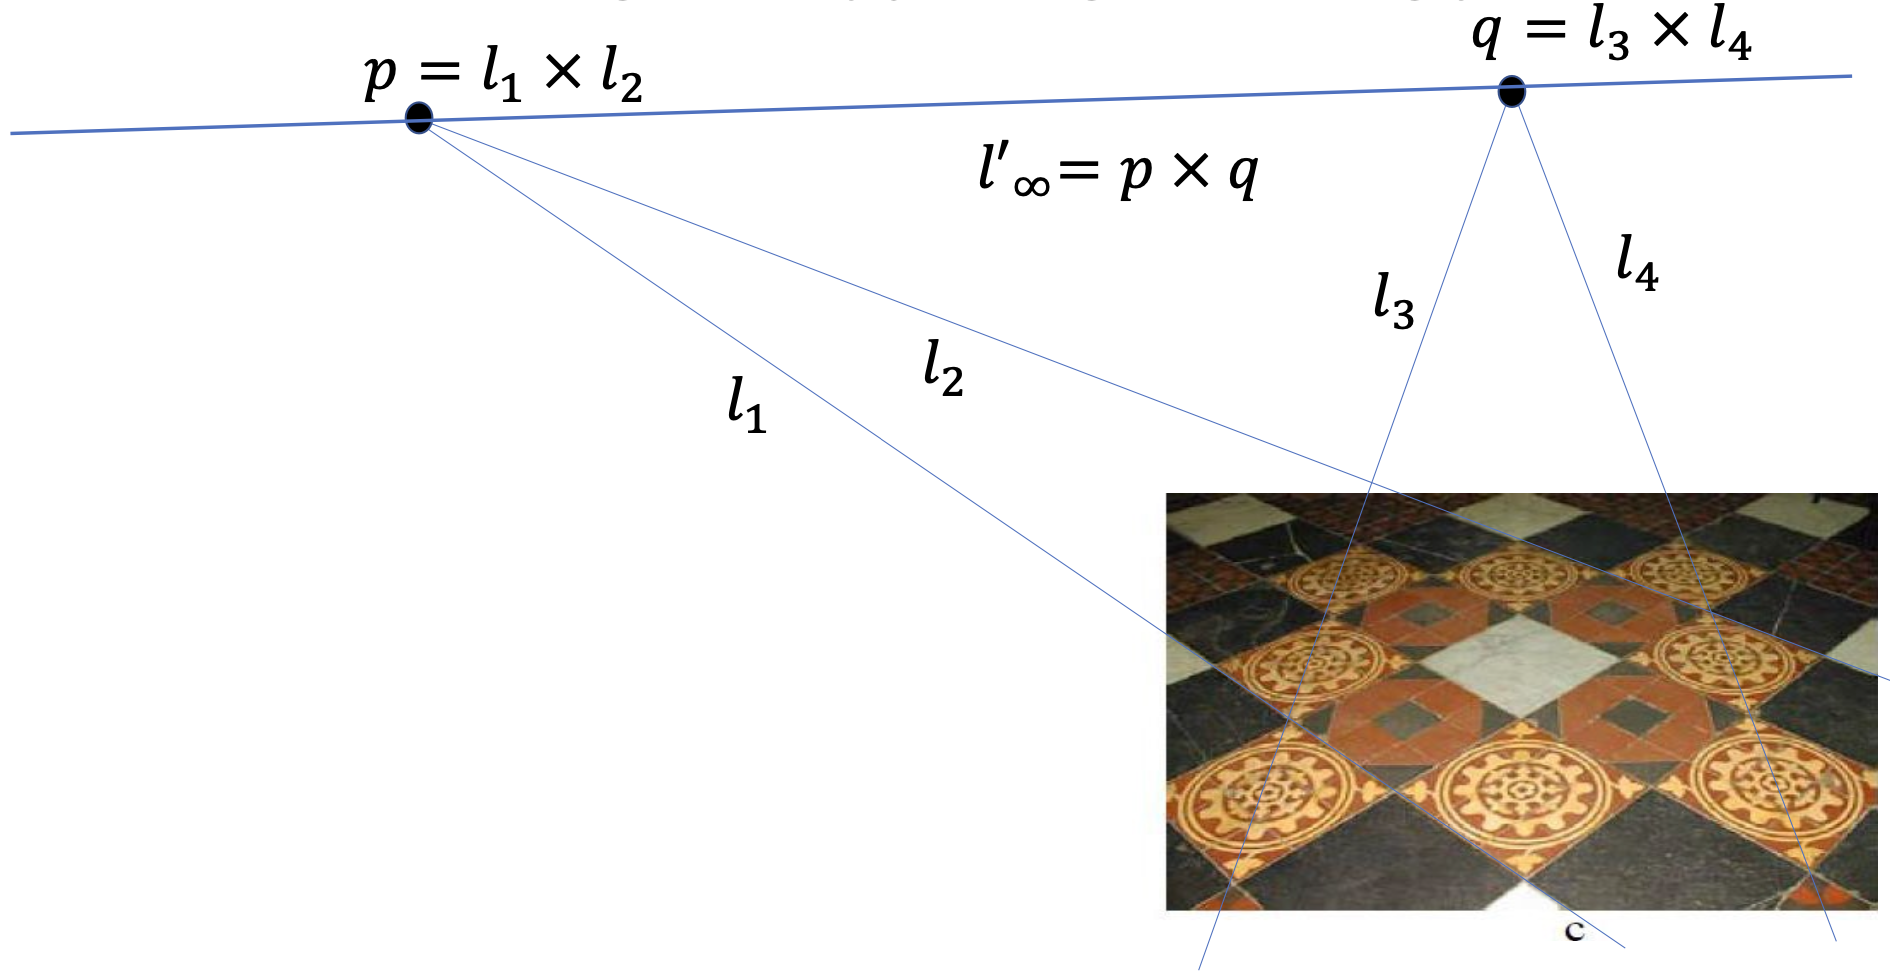
\includegraphics[width=0.5\linewidth]{images/van.png}
            \end{figure}
    \end{itemize}

    \subsection{Shape reconstruction}
    \begin{theorem}
        A projective transformation $H$ maps the circular points $\boldsymbol{I}$ and $\boldsymbol{J}$ onto themselves implies that and 
        implies from $H$ is a similarity. 
    \end{theorem}
    \begin{proof}
        Multiplying a similarity matrix $H_S$ by circular point $\boldsymbol{I}$, a multiple of $\boldsymbol{I}$ is obtained. Analogous 
        result is obtained for the other circular point $\boldsymbol{J}$. 
    \end{proof}
    The given image is a general projective mapping of the original scene. So, the image $(\boldsymbol{I}^{'},\boldsymbol{J}^{'})$ of 
    circular points $()\boldsymbol{I},\boldsymbol{J}$ of the scene plane is in general different from $\boldsymbol{I},\boldsymbol{J}$.
    We can use $\boldsymbol{I}^{'},\boldsymbol{J}^{'}$ as additional information: if we apply to the image a new projective
    mapping $H_{SR}$ which maps $\boldsymbol{I}^{'},\boldsymbol{J}^{'}$ back to $\boldsymbol{I},\boldsymbol{J}$, we obtain a new, 
    modified image. The new image of the circular points $\boldsymbol{I},\boldsymbol{J}$ is again $\boldsymbol{I},\boldsymbol{J}$. 
    So, from the theorem, the obtained model (new image) is similar to the original scene. We have that the obtained model is a shape 
    reconstruction of the scene. 
    \begin{figure}[H]
        \centering
        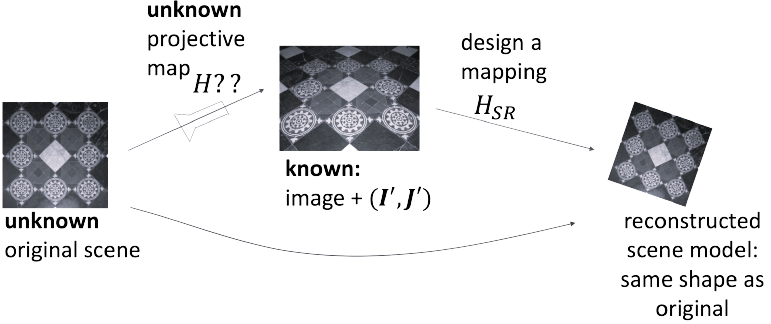
\includegraphics[width=0.75\linewidth]{images/HSR.png}
    \end{figure}
    The issues with this method are: 
    \begin{itemize}
        \item Find a projective mapping $H_{SR}$ which maps $\boldsymbol{I}^{'},\boldsymbol{J}^{'}$ back to 
            $\boldsymbol{I},\boldsymbol{J}$: finding one of the $\infty^{4}$ matrices such that: 
            $\begin{cases}
                H_{SR}\boldsymbol{I}^{'}=\boldsymbol{I} \\
                H_{SR}\boldsymbol{J}^{'}=\boldsymbol{J}
            \end{cases}$. Let us use equivalent information instead: the degenerate conic dual to $\boldsymbol{I}^{'},\boldsymbol{J}^{'}$, 
            that is $C_{\infty}^{'*}=\boldsymbol{I}^{'}\boldsymbol{J}^{'T}+\boldsymbol{J}^{'}\boldsymbol{I}^{'T}$. This dual conic is the 
            image of the original conic dual to the circular points $(\boldsymbol{I},\boldsymbol{J})$: 
            \[C_{\infty}^{*}=\boldsymbol{I}\boldsymbol{J}^{T}+\boldsymbol{J}\boldsymbol{I}^{T}\]
            in fact, since $(\boldsymbol{I}^{'},\boldsymbol{J}^{'})$ is the image of $(\boldsymbol{I},\boldsymbol{J})$, then also 
            $C_{\infty}^{'*}$ is the image of $C_{\infty}^{*}$. So, any projectivity $H_{SR}$ which maps $(\boldsymbol{I}^{'},\boldsymbol{J}^{'})$
            back to $(\boldsymbol{I},\boldsymbol{J})$ also maps $C_{\infty}^{'*}$ back to $C_{\infty}^{*}$. Using the transformation rule for dual 
            conics under projective mappings we get: 
            \[C^{*}_{\infty}=H_{SR}C^{'*}_{\infty}H_{SR}^T\]
            Inverting this relationship yields: 
            \[C_{\infty}^{'*}=H_{SR}^{-1} 
            \begin{bmatrix}
                1 & 0 & 0 \\
                0 & 1 & 0 \\
                0 & 0 & 0
            \end{bmatrix}
            H_{SR}^{-T}\]
            If we apply the singular value decomposition to this equation we obtain that the matrices $H_{SR}^{-1}$ and $H_{SR}^{-T}$ are
            perpendicular, so: 
            \[SVC(C_{\infty}^{'*})=U_\perp
            \begin{bmatrix}
                1 & 0 & 0 \\
                0 & 1 & 0 \\
                0 & 0 & 0
            \end{bmatrix}
            U_{\perp}^T\]
            This provides exactly one solution: $H_{SR}=U_{\perp}^{-1}=U_{\perp}^T$
        \item Find the vanishing line: it is possible to use additional knowledge items, such as the image of parallel lines. 
            \begin{figure}[H]
                \centering
                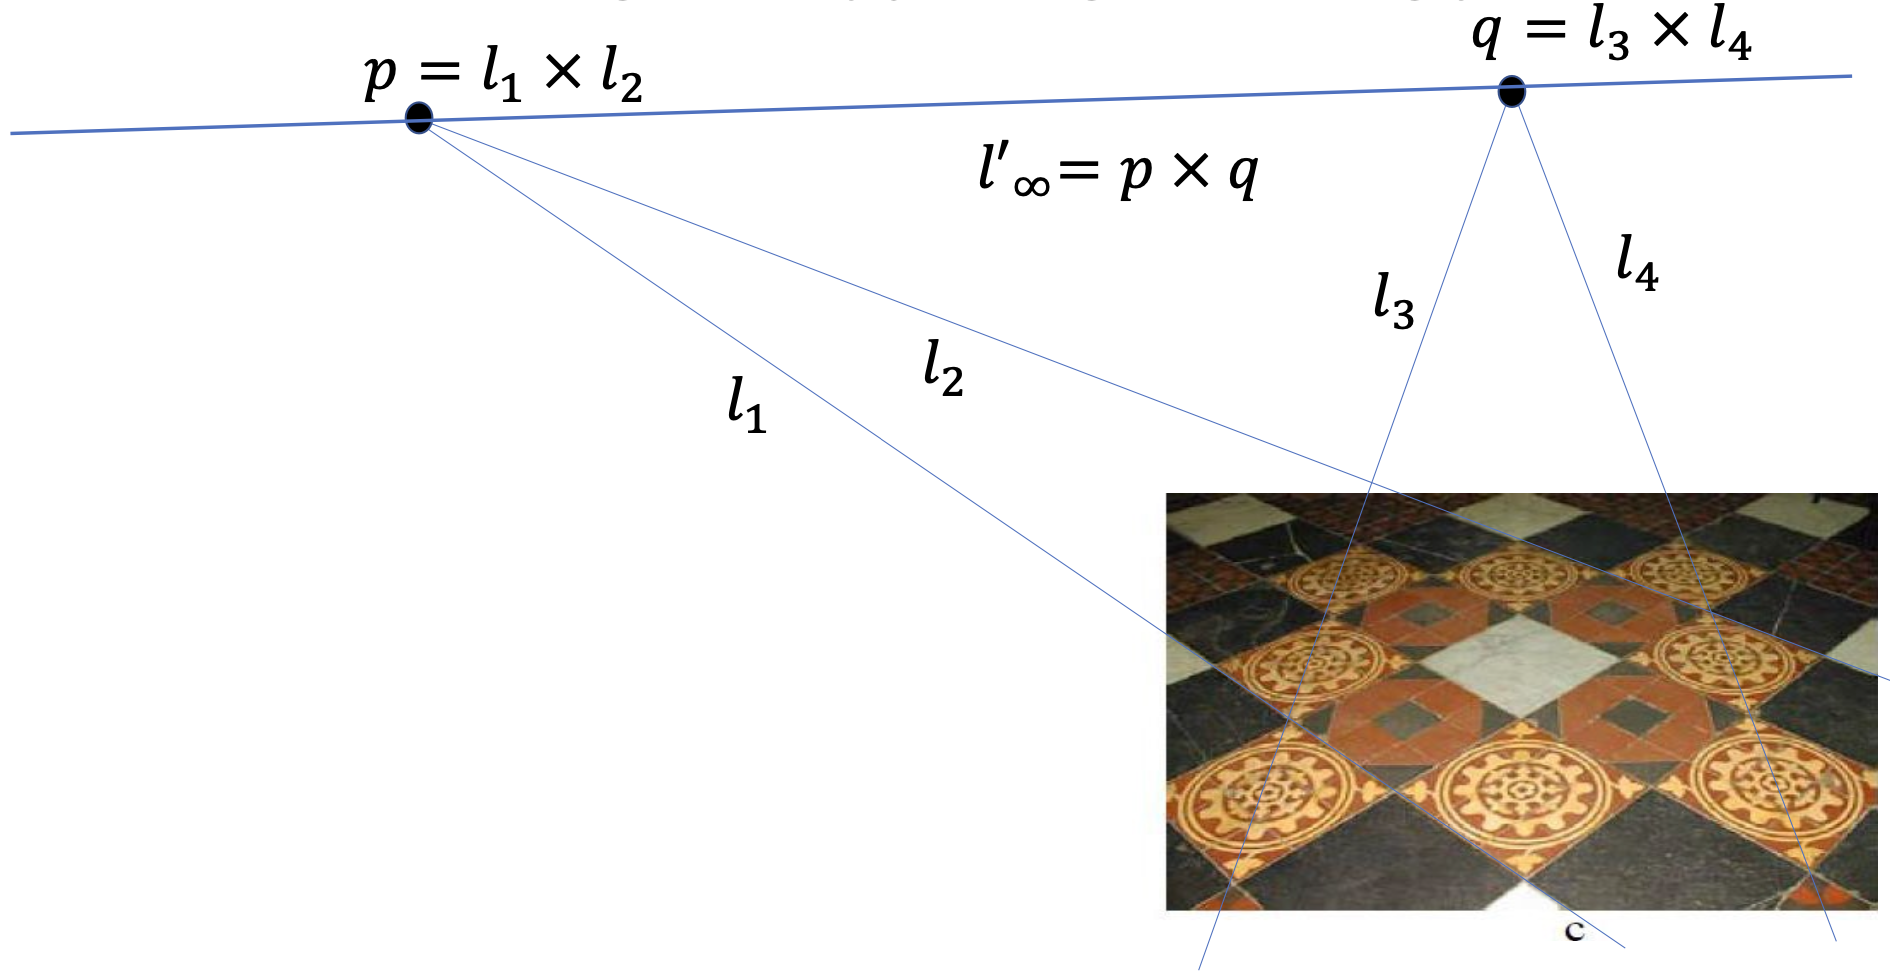
\includegraphics[width=0.5\linewidth]{images/van.png}
            \end{figure}
    \end{itemize}





\end{document}